% Title: Report LaTex File: Concept Development
% Auther: DC Eksteen
% Student Number: 22623906
% Contact: 22623906@sun.ac.za
% Date: 2022/09/22
% Version: 2.0

\chapter{Concept Design and Evaluation}
\label{ch:concept}
% Section overview:

In this chapter the engineering requirements are identified and refined. The final selected concept is then proposed and analysed against the determined requirements. The content presented in this chapter has been refined through many iterations and present the final outcome of the conceptualisation process.

In order to avoid confusion, some commonly used terms are defined in Appendix~\ref{sec:defs3}.

Table~\ref{tab:conditions} presents the user requirements that were derived from the project objectives and the literature review.

\begin{table}[H]
	%\renewcommand{\arraystretch}{\tablestretch}
	\centering
	\caption{Derived User Requirements}
	\begin{tabularx}{\textwidth}{>{\raggedright UR~}p{1.5 cm} X >{\raggedright\arraybackslash}p{2cm}}
		\toprule
		\multicolumn{2}{c}{User Requirement} & Priority                                                   \\
		\midrule
		\newR{UR:zwift}                      & Connect with Zwift                             & Essential \\
		\newR{UR:sim}                        & Realistic Riding Simulation                    & Essential \\
		\newR{UR:weight}                     & Weight Should be Comparable to Market Products & High      \\
		\newR{UR:range}                      & Accept a Wide Range of Bicycles                & High      \\
		\newR{UR:measure}                    & Accurate Measured Training Data                & Medium    \\
		\newR{UR:price}                      & Less Expensive than Market Products            & High      \\
		\newR{UR:store}                      & Platform Easily Stored                         & Medium    \\
		\bottomrule
	\end{tabularx}
	\label{tab:conditions}
\end{table}

\vspace*{-0.5cm}

\setcounter{reqCount}{0}

\section{Requirement Analysis}
\label{sec:req}

Table~\ref{tab:funcreq} shows the functional requirements that were determined from the user requirements in Table~\ref{tab:conditions}.

\begin{table}[H]
	\renewcommand{\arraystretch}{\tablestretch}
	\centering
	\caption{Functional Engineering Requirements}
	\begin{tabularx}{\textwidth}{>{\raggedright FR~}p{0.8 cm} X >{\centering\arraybackslash}p{1.7cm}}
		\toprule
		\multicolumn{2}{c}{Functional Requirement} & Reference                                                                                 \\
		\midrule
		\newR{FR:ble}                              & Have \ac{ble} or ANT+ Connectivity                                  & UR \ref{UR:zwift}   \\
		\newR{FR:wheel}                            & \capitalisefmtwords{Accommodate both 27.5' and 29' wheel diameters} & UR \ref{UR:range}   \\
		\newR{FR:speed}                            & \capitalisefmtwords{Be Able to Determine Wheel Speed}               & UR \ref{UR:measure} \\
		\newR{FR:func}                             & \capitalisefmtwords{perform training sessions on Zwift application} & UR \ref{UR:sim}     \\
		\bottomrule
	\end{tabularx}
	\label{tab:funcreq}
\end{table}

\vspace*{-0.5cm}

\setcounter{reqCount}{0}

Table~\ref{tab:perfreq} contains the performance measures that are used to measure the success of developed concepts.

\begin{table}[H]
	\renewcommand{\arraystretch}{\tablestretch}
	\centering
	\caption{Performance Engineering Requirements}
	\begin{tabularx}{\textwidth}{>{\raggedright PR~}p{0.8 cm} X p{1.1cm} p{1.6cm} p{1cm} >{\centering\arraybackslash}p{1.7cm}}
		\toprule
		\multicolumn{2}{c}{Performance Requirement} & Target                 & Value & Unit     & Reference                                      \\
		\midrule
		\newR{PR:wheelbase}                         & Allowable Wheelbase    & Range & 900-1200 & \si{\milli\meter}         & UR~\ref{UR:range}  \\
		\newR{PR:weight}                            & Weight                 & Max   & 8        & \si{\kilogram}            & UR~\ref{UR:weight} \\
		\newR{PR:speed}                             & Simulated Moving Speed & Range & 10-50    & \si{\kilo\meter\per\hour} & UR~\ref{UR:sim}    \\
		\newR{PR:27speed}                           & Wheel Speed (27.5')    & Range & 82-408   & \ac{rpm}                  & UR \ref{UR:sim}    \\
		\newR{PR:29speed}                           & Wheel Speed (29')      & Range & 76-379   & \ac{rpm}                  & UR \ref{UR:sim}    \\
		\newR{PR:power}                             & Braking Force          & Range & 0.5-4.5  & \si{\newton}              & UR \ref{UR:sim}    \\
		\bottomrule
	\end{tabularx}
	\label{tab:perfreq}
\end{table}

\vspace*{-0.5cm}

\label{sec:opspeedc}


\section{System Context}
\label{sec:conc}

The distinction between the \ac{nsoi}, \ac{wsoi} and the environment was defined in order to determine the scope and boundaries of the project.

Elements contained within the \ac{wsoi} are independent of the concept and cannot be changed by the solution. These \ac{wsoi} elements interact directly with the \ac{nsoi} during its normal operation cycle. Elements are classified as the environment when they may have an influence on the \ac{nsoi}, but will not be affected by the \ac{nsoi} during normal operation. The proposed boundaries between the system elements is shown in Figure~\ref{fig:soi}.

\begin{figure}[H]
	\begin{center}
		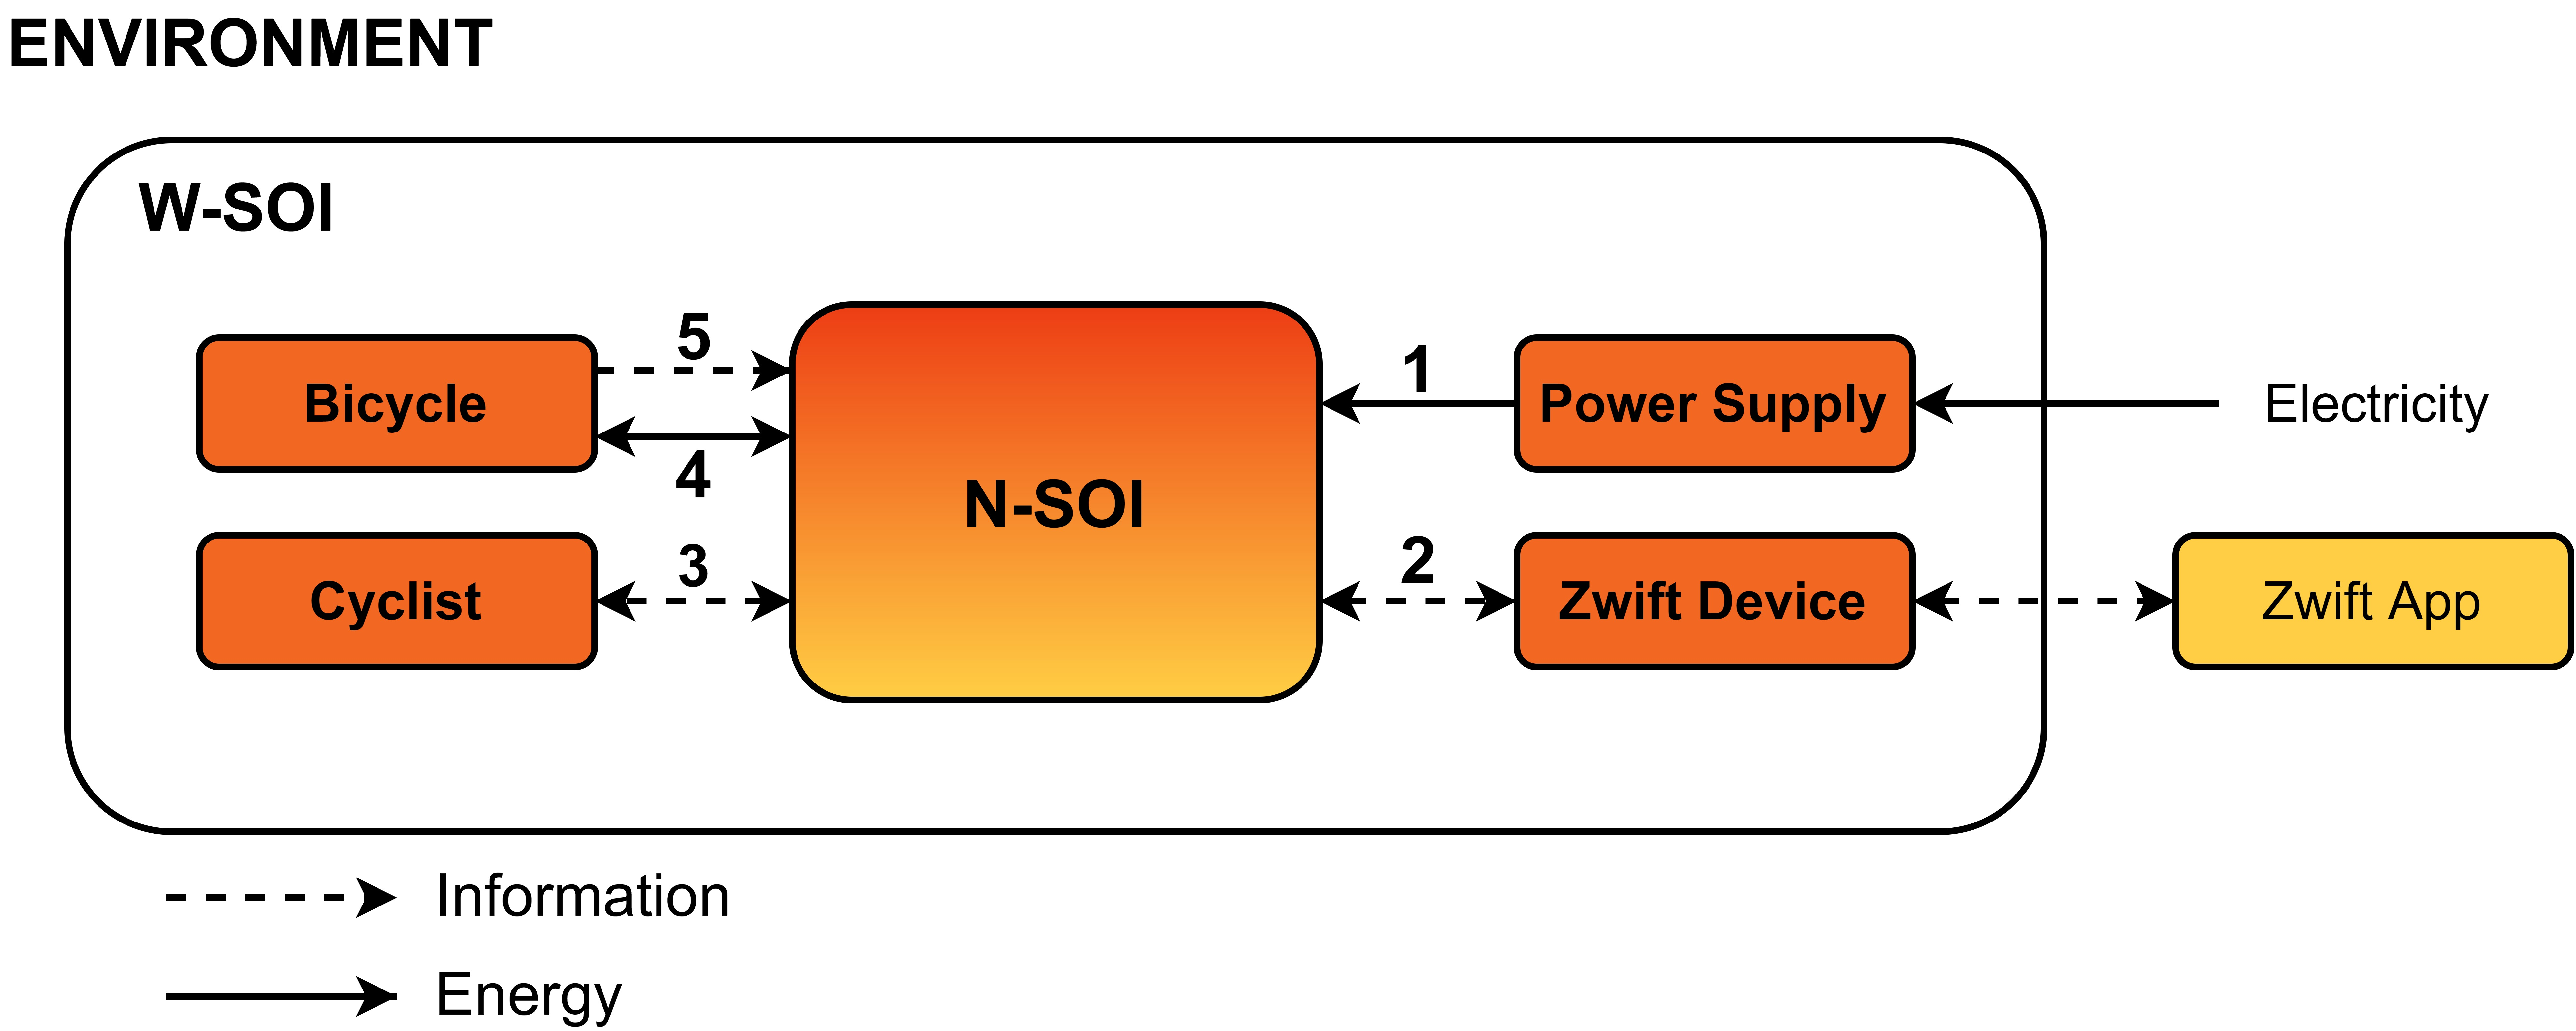
\includegraphics[width=\textwidth]{SOI.jpg}
		\caption{Concept Boundary}
		\label{fig:soi}
	\end{center}
\end{figure}

Table~\ref{tab:links} defines the interfaces between the elements in Figure~\ref{fig:soi}. At this point Interface 2 defines that \ac{ble} technology will be used as communication protocol. This aims to achieve a more robust solution that will allow for far more development potential in the future and the decision is explained in more detail in Appendix~\ref{sec:defs3}

\begin{table}[H]
	\renewcommand{\arraystretch}{\tablestretch}
	\centering
	\caption{Concept Boundary Interfaces}
	\begin{tabularx}{\textwidth}{p{1.5cm} X p{3.5cm}}
		\toprule
		Interface & Description                             & Type              \\
		\midrule
		1         & Power delivery to platform              & Electrical Energy \\
		2         & \ac{ble} with \ac{ftms} implementation  & Information       \\
		3         & Communication between user and platform & User Info         \\
		4         & Resistance applied to bicycle           & Energy Losses     \\
		5         & Sensor readings of cycling data         & Sensor Info       \\
		\bottomrule
	\end{tabularx}
	\label{tab:links}
\end{table}

\section{\ac{nsoi} Selection}

After considering all types of trainers mentioned in Section~\ref{sec:train}, roller trainers were selected as the platform that will achieve the most desirable outcome. For applying the controllable resistance, an eddy current brake was selected to be implemented on the roller trainers. Speed sensors on the rollers would allow the system to determine the cycling speed and a \ac{ble} transceiver module would enable communication with the device hosting the Zwift application.

\subsubsection{Roller Trainer}

Roller trainers are the most robust platform, allowing any type of bicycle to be used on them. It is not required to remove, alter or add to any parts of existing bicycles. Roller trainers have the added benefit of being less complicated to manufacture than other types of trainers, and are maintainable without requiring proprietary parts. There are many examples of consumers creating their own roller trainers on the internet, yet there are a very limited amount of commercially available roller trainers with smart connectivity.

Roller trainers require a higher level of skill to use, as the bicycle is not fixed to the trainer and the cyclist thus needs to balance the bicycle during operation. The trainer can be designed to be compact to store, easy to operate and inexpensive to manufacture and maintain. Most of the components of the trainer can be manufactured or assembled using commonly available materials and parts.

\subsubsection{Eddy Current Brake}

The resistance of the platform will be controlled by an eddy current brake attached to one of the rollers of the trainer. An eddy current brake was selected for its maintenance free operation and repeatable control.

The diameter ratio between the bicycle wheels and the rollers will also allow for higher operating speeds of the eddy current brake. The braking torque applied by the brake will be converted into heat. Active cooling might be required if the excess heat cannot be dissipated into the environment rapidly enough.

\subsubsection{Software Overview}

Control and communication functions of the system will be handled by a Raspberry Pi micro controller. This will allow for integration between the selected hardware and electronics with the developed communications software. Since the software was developed independently of the selected system, some integration would be required to allow compatibility with the Zwift application.

\section{Concept Evaluation}
\label{sec:eval}

In order to ensure that all engineering requirements are met by the proposed concept, Table~\ref{tab:eval} indicates the proposed solution to each of the requirements that have been identified in Table~\ref{tab:funcreq} and Table~\ref{tab:perfreq}.

\begin{table}[H]
	\renewcommand{\arraystretch}{\tablestretch}
	\centering
	\caption{Concept Requirement Fulfilment Analysis}
	\begin{tabularx}{\textwidth}{p{2cm} >{\raggedright\arraybackslash}X}
		\toprule
		Target                & \multicolumn{1}{c}{Proposed Solution}                                                   \\
		\midrule
		FR~\ref{FR:ble}       & {Raspberry Pi with integrated or external \ac{ble} module.}                             \\
		FR~\ref{FR:wheel}     & {Roller trainers allow for wide range of wheel diameters.}                              \\
		FR~\ref{FR:speed}     & {Speed sensors implemented on rollers.}                                                 \\
		FR~\ref{FR:func}      & {Rollers are proven technology. Smart connectivity will allow for Zwift compatibility.} \\
		PR~\ref{PR:wheelbase} & {Rollers often allow for adjustable wheelbase lengths.}                                 \\
		PR~\ref{PR:weight}    & {Rollers do not require any bicycle mounting components.}                               \\
		PR~\ref{PR:speed}     & {Rollers do not limit the operating speed.}                                             \\
		PR~\ref{PR:27speed}   & {Rollers function independent of bicycle wheel diameter.}                               \\
		PR~\ref{PR:29speed}   & {Rollers function independent of bicycle wheel diameter.}                               \\
		PR~\ref{PR:power}     & {Eddy current brake applied to rear roller controller from Raspberry~Pi.}               \\
		\bottomrule
	\end{tabularx}
	\label{tab:eval}
\end{table}